\documentclass[../piano-di-progetto.tex]{subfiles}
\begin{document}

\subsection{Codifica di dettaglio}
Il periodo di codifica di dettaglio inizia il 2020-05-18, dopo la revisione di progettazione, e termina il giorno 2020-06-18 con la terza revisione di avanzamento.
\subsubsection{Ruoli}
Durante questa macro, viene richiesta la presenza dei seguenti ruoli:
\begin{itemize}
    \item Responsabile;
    \item Amministratore;
    \item Progettista;
    \item Verificatore.
\end{itemize}

\subsection{Attività}
Per semplicità, questa macro viene suddivisa in periodi:

\begin{itemize}
    \item \textbf{I periodo (2020-05-18 2020-06-10)}: vengono effettuati cinque incrementi per la realizzazione di una \glossario{product baseline}, verranno illustrati nella prossima sottosezione;
    \item \textbf{II periodo (2020-06-11 2020-06-17)}:
        \begin{itemize}
            \item Preparazione della presentazione;
            \item Verifica.
        \end{itemize}
\end{itemize}
\subsection{Incrementi}

\subsubsection{V incremento}
\emph{2020-05-18 - 2020-05-21}. 
 
 Vengono stabiliti i seguenti obiettivi per l'incremento:
 \begin{itemize}
     \item Implementazione dell'algoritmo di SVM per la generazione dei predittori nel programma di addestramento;
 \end{itemize}

Durante l'incremento verranno svolte le seguenti attività: 
\begin{itemize}
    \item Progettazione;
    \item Codifica;
    \item Verifica.
\end{itemize}

\subsubsection{VI incremento}
\emph{2020-05-22 - 2020-05-26}. 
 
 Vengono stabiliti i seguenti obiettivi per l'incremento:
 \begin{itemize}
     \item Implementazione del caricamento dei predittori nel plug-in;
     \item Implementazione della possibilità di scegliere nel plug-in i nodi su cui effettuare predizioni.
 \end{itemize}

Durante l'incremento verranno svolte le seguenti attività: 
\begin{itemize}
    \item \textbf{Progettazione};
    \item \textbf{Codifica};
    \item \textbf{Stesura del manuale};
    \item \textbf{Verifica};
\end{itemize}

\subsubsection{VII incremento}
\emph{2020-05-27 - 2020-06-02}. 
 
 Vengono stabiliti i seguenti obiettivi per l'incremento:
 \begin{itemize}
    \item Implementazione delle predizioni del plug-in;
    \item Implementazione del collegamento tra predizioni e front-end.

\end{itemize}

Durante l'incremento verranno svolte le seguenti attività: 
\begin{itemize}
    \item Progettazione;
    \item Codifica;
    \item Stesura del manuale;
    \item Verifica.
\end{itemize}

\subsubsection{VIII incremento}
\emph{2020-06-03 - 2020-06-06}. 
 
 Vengono stabiliti i seguenti obiettivi per l'incremento:
 \begin{itemize}
    \item Implementazione della gestione degli errori;
    \item Implementazione delle impostazione per la rimozione del plug-in;

 \end{itemize}

Durante l'incremento verranno svolte le seguenti attività: 
\begin{itemize}
    \item Progettazione;
    \item Codifica;
    \item Stesura del manuale;
    \item Verifica.
\end{itemize}

\subsubsection{IX incremento}
\emph{2020-06-07 - 2020-06-10}. 
 
 Vengono stabiliti i seguenti obiettivi per l'incremento:
 \begin{itemize}
    \item Implementazione delle impostazione degli alert;
    \item Implementazione della possibilità di applicare la trasformazione logaritmica nel programma di addestramento;
    \item Implementazione della possibilità di applicare la trasformazione esponenziale nel programma di addestramento.

 \end{itemize}

Durante l'incremento verranno svolte le seguenti attività: 
\begin{itemize}
    \item Progettazione;
    \item Codifica;
    \item Stesura del manuale;
    \item Verifica.
\end{itemize}



\newpage
\begin{landscape}
    \begin{figure}[H]
        \centering
        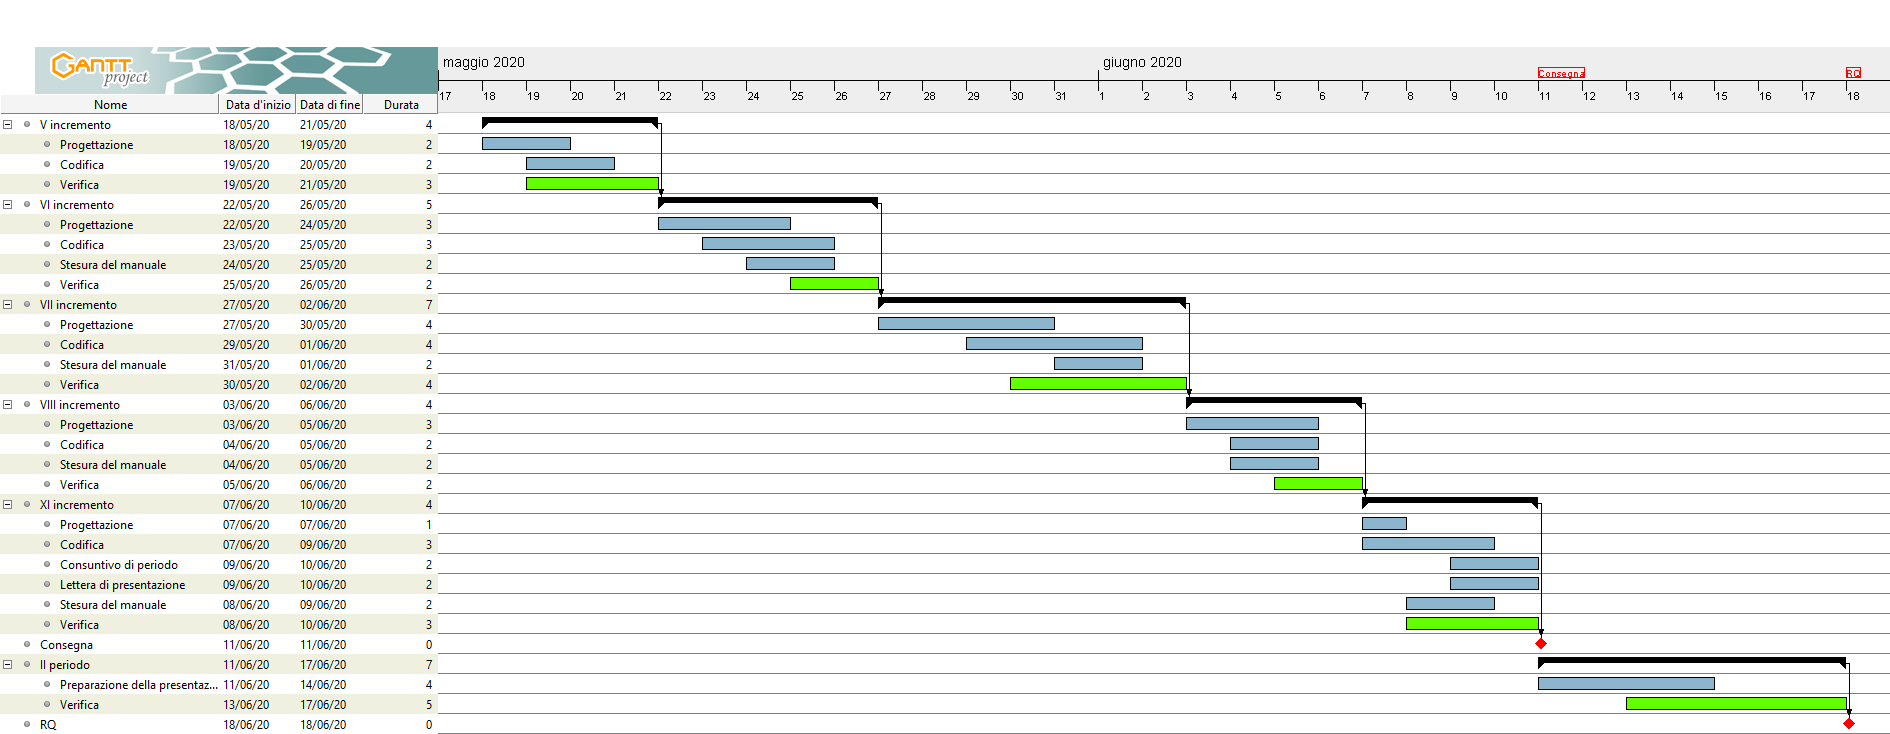
\includegraphics[width=24cm]{img/codifica.png}
        \caption{Diagramma attività nel periodo di codifica di dettaglio}
      \end{figure}
\end{landscape}

\end{document}
